\section{Kemajuan Penelitian}
\subsection{Teknologi Pendukung}

\begin{frame}{Teknologi Pendukung}
  \begin{columns}[t]
    \begin{column}{.5\linewidth}
      Ada beberapa teknologi dalam mendukung penelitian yang dilakukan, diantaranya:
      \begin{itemize}
        \item XFLR5
        \item Python
        \item Django
        \item Vue.js
        \item PostgreSQL
      \end{itemize}
    \end{column}
    \begin{column}{.5\linewidth}
      \begin{figure}[h]
        \centering
        
\includegraphics[width=0.6\linewidth]{statics/stacks}
        \caption{Teknologi \textit{open source}}
        \label{fig:opentek}
      \end{figure}
    \end{column}
  \end{columns}
\end{frame}

\subsection{Fitur Aplikasi}
\begin{frame}{Pencitraan Airfoil}
  \begin{figure}[h]
    \centering
    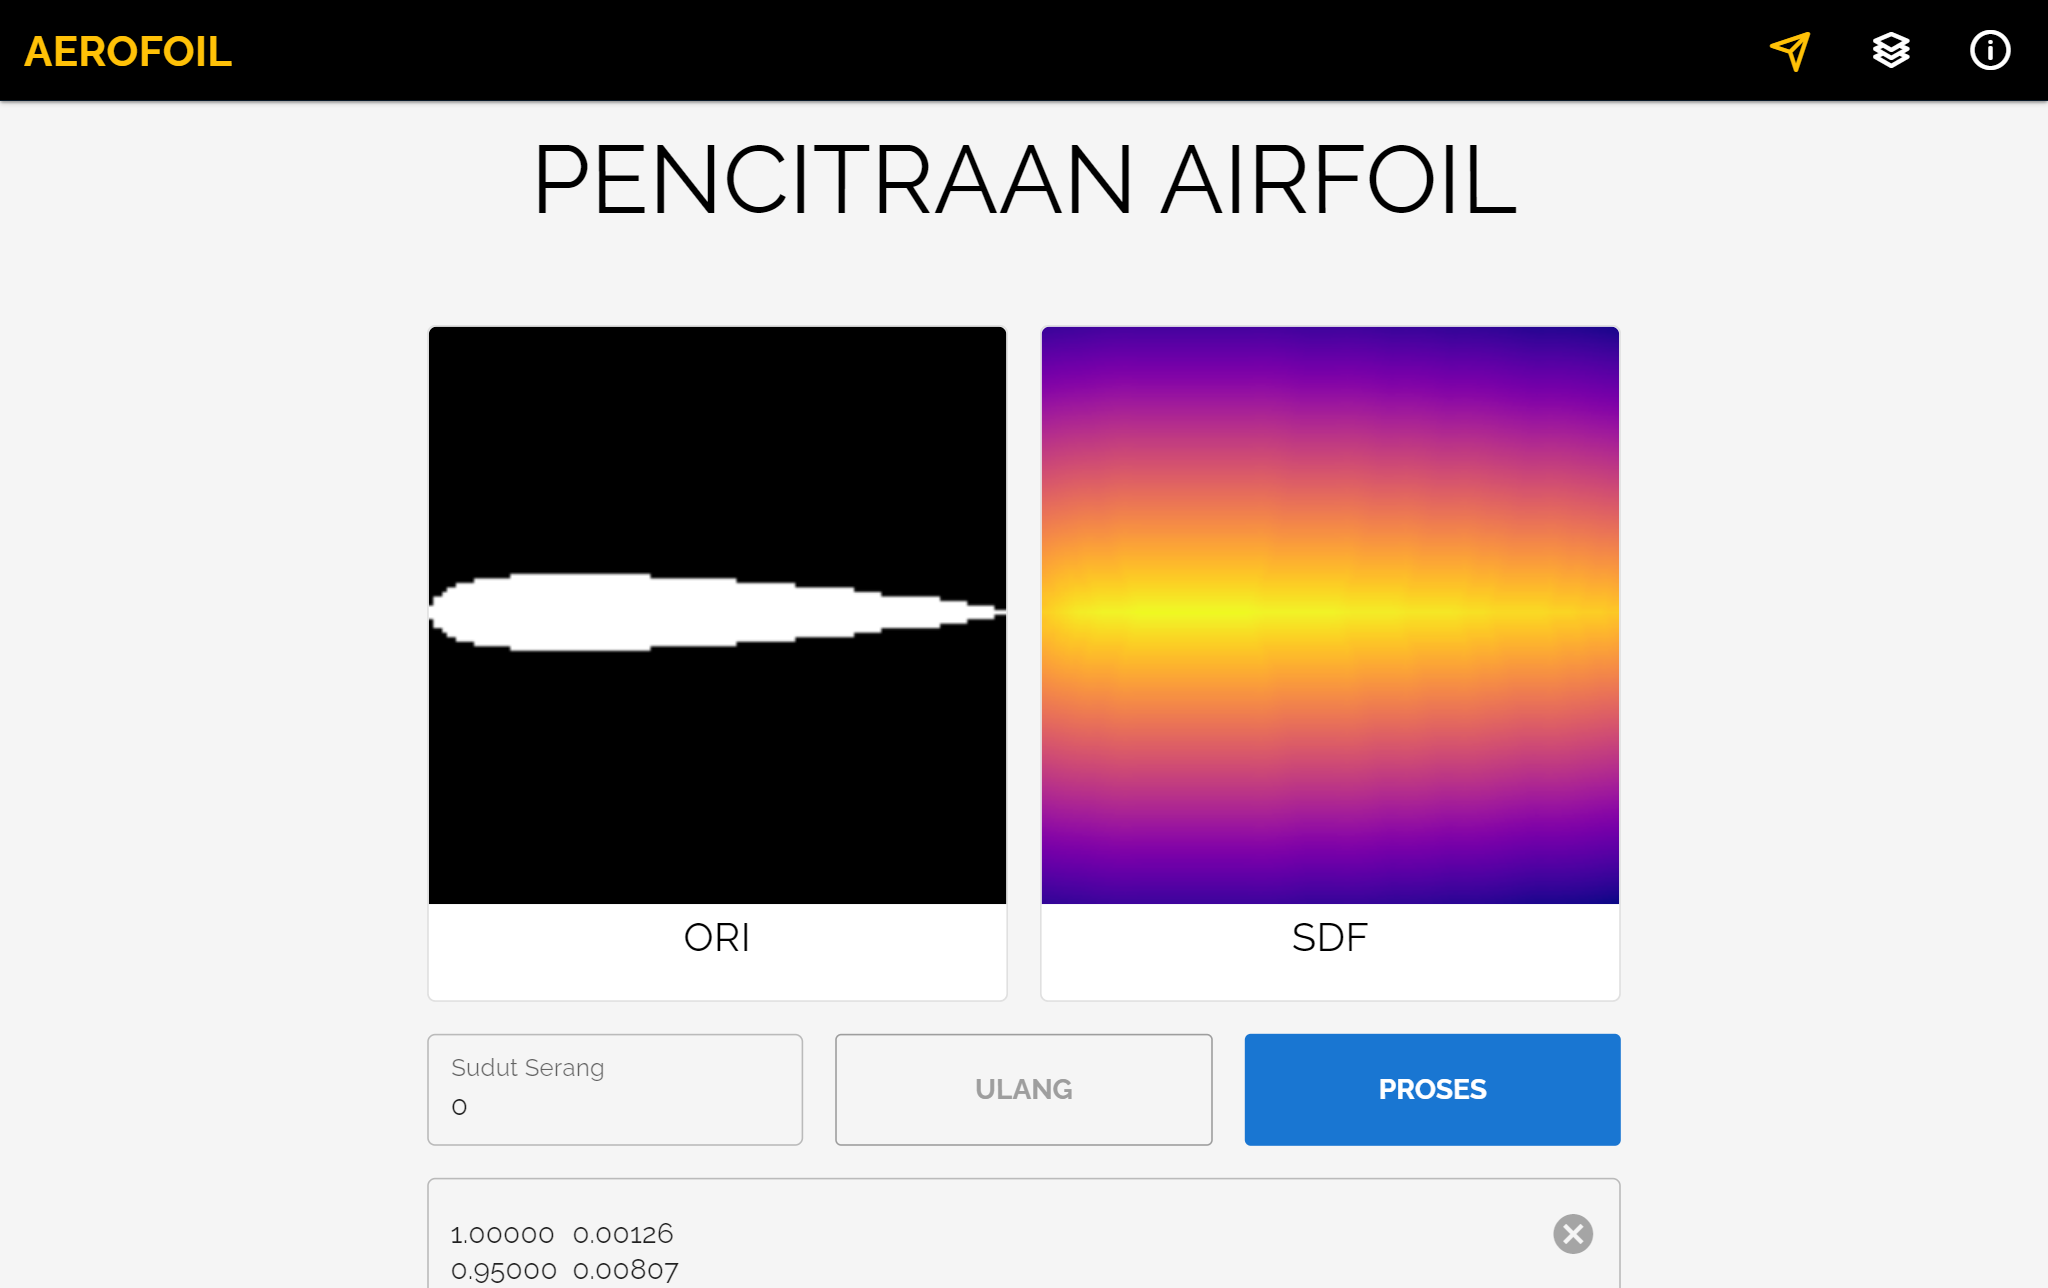
\includegraphics[width=0.7\linewidth]{statics/citra_airfoil}
  \end{figure}
\end{frame}

\begin{frame}{Koleksi Data Aerodinamika Airfoil}
  \begin{figure}[h]
    \centering
    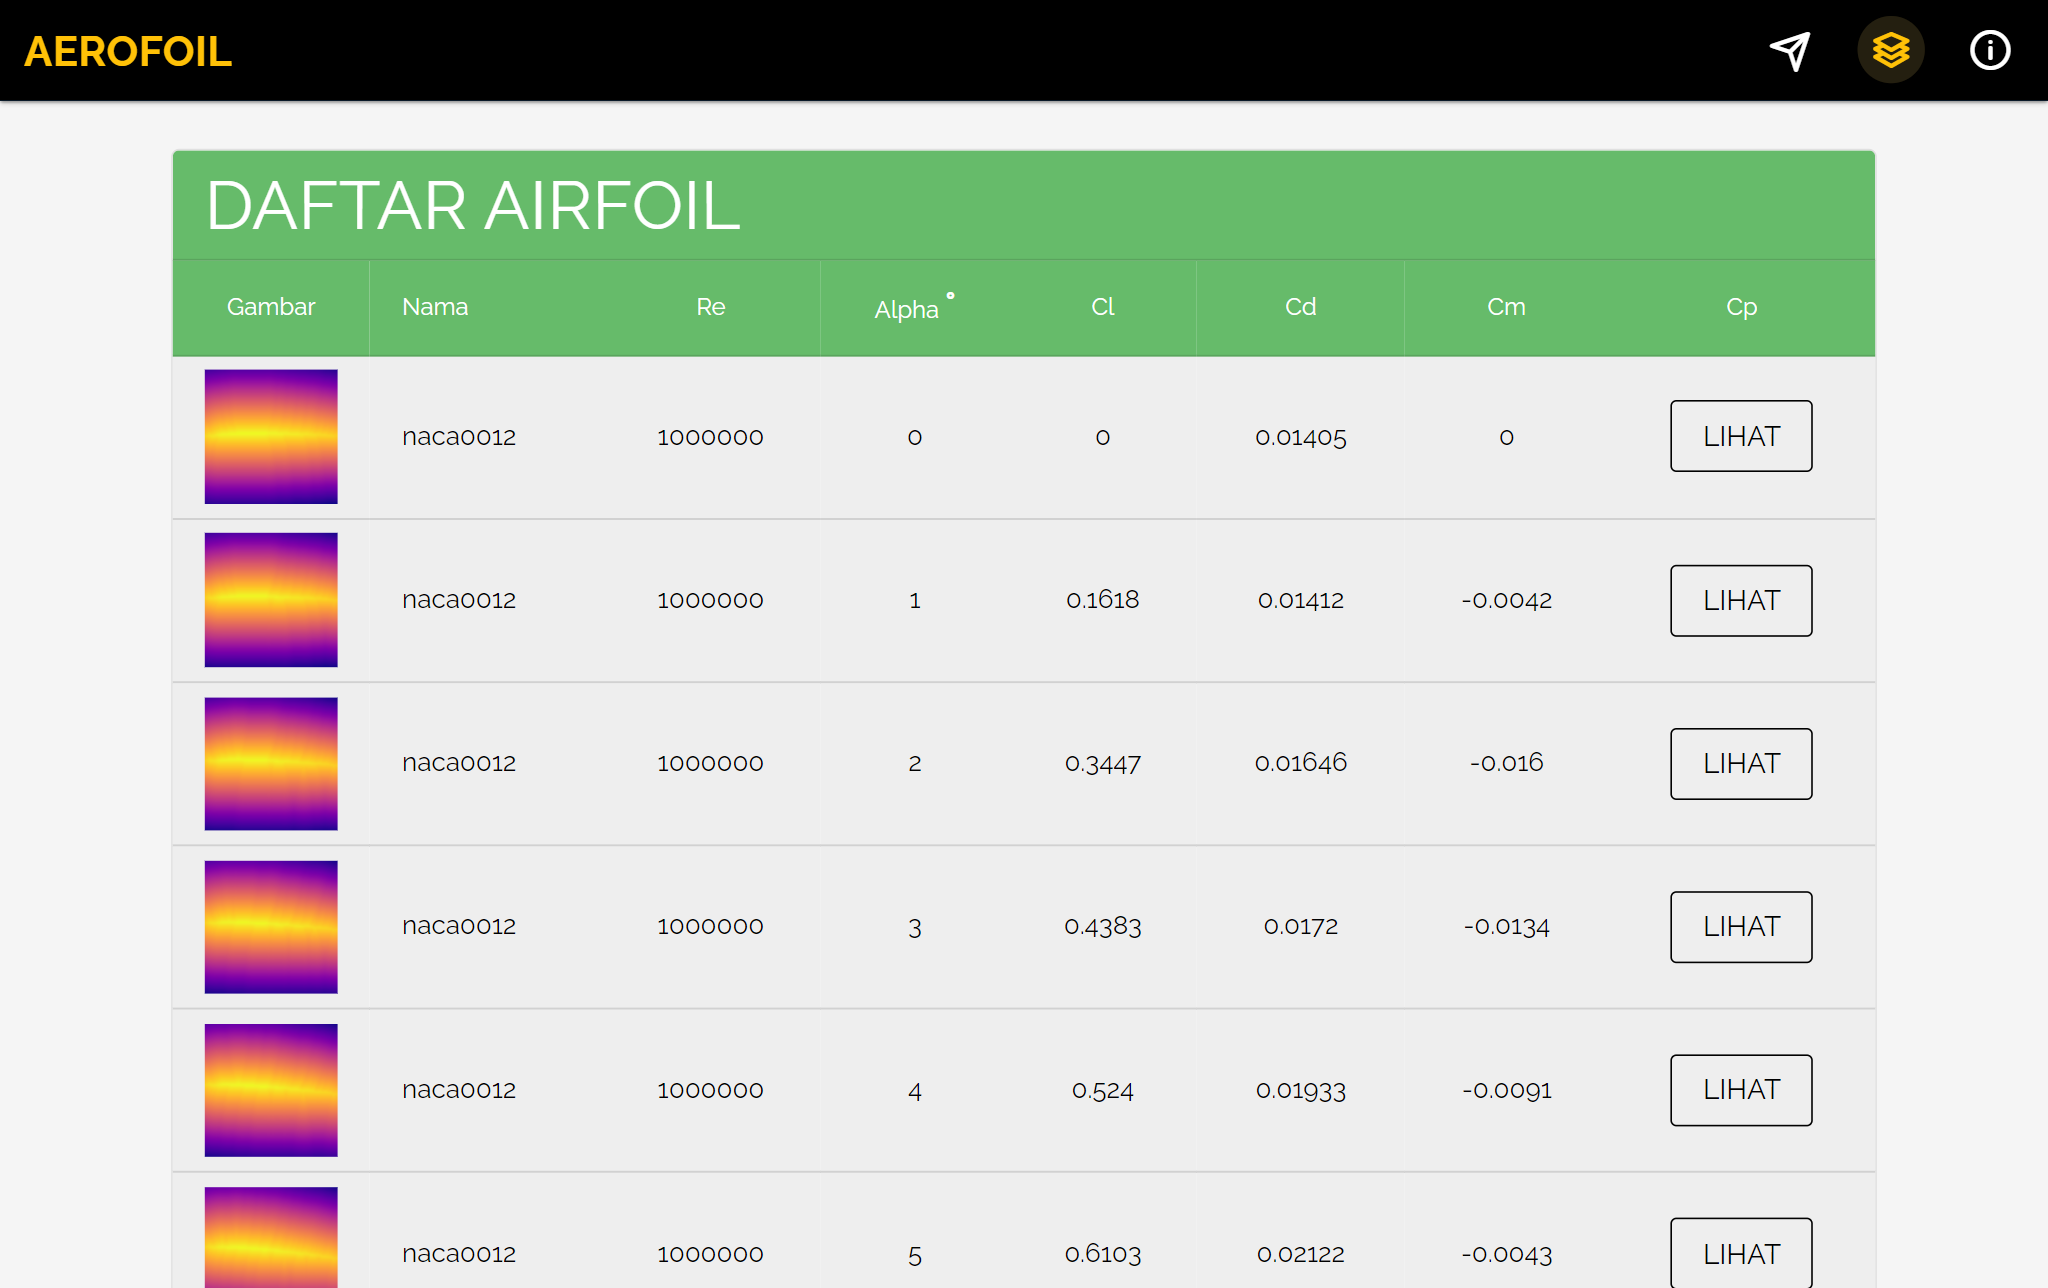
\includegraphics[width=0.7\linewidth]{statics/aerodinamika_airfoil}
  \end{figure}
\end{frame}

\begin{frame}{Otomasi SDF Airfoil melalui \textit{CLI}}
  \begin{block}{Memanfaatkan \textit{Multiprocessing}}
    Diharapkan dapat membantu mempercepat SDF airfoil
  \end{block}

  \begin{block}{Instruksi di \textit{Console}}
    \texttt{python manage.py autosdf naca0012 coord.csv 0 5 10 15}
  \end{block}

  \begin{columns}[t]
    \begin{column}{.25\linewidth}
      \begin{figure}[h]
        \centering
        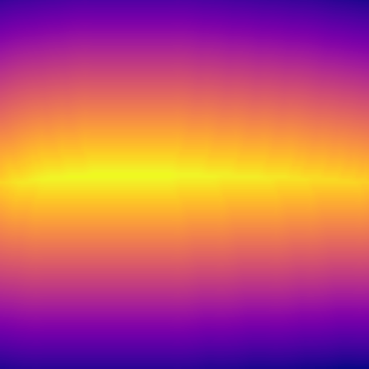
\includegraphics[width=0.5\linewidth]{statics/naca0012_0.0}
        \caption{$0^\circ$}
      \end{figure}
    \end{column}

    \begin{column}{.25\linewidth}
      \begin{figure}[h]
        \centering
        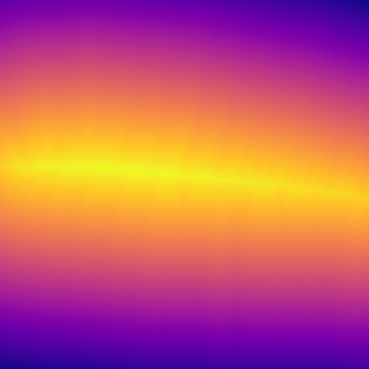
\includegraphics[width=0.5\linewidth]{statics/naca0012_5.0}
        \caption{$5^\circ$}
      \end{figure}
    \end{column}

    \begin{column}{.25\linewidth}
      \begin{figure}[h]
        \centering
        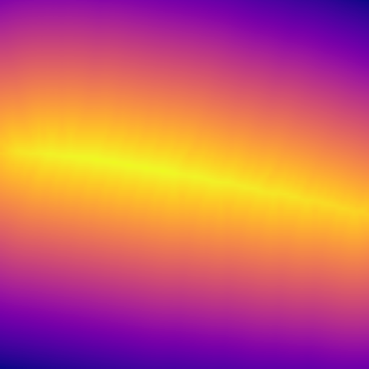
\includegraphics[width=0.5\linewidth]{statics/naca0012_10.0}
        \caption{$10^\circ$}
      \end{figure}
    \end{column}

    \begin{column}{.25\linewidth}
      \begin{figure}[h]
        \centering
        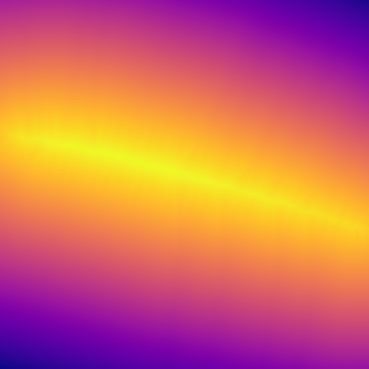
\includegraphics[width=0.5\linewidth]{statics/naca0012_15.0}
        \caption{$15^\circ$}
      \end{figure}
    \end{column}
  \end{columns}
\end{frame}

\begin{frame}{Otomasi Simpan Data Aerodinamika Airfoil melalui \textit{CLI}}
  \begin{block}{Instruksi di \textit{Console}}
    \texttt{python manage.py autodb aero.txt naca0012 1000000}
  \end{block}

  \begin{figure}[h]
    \centering
    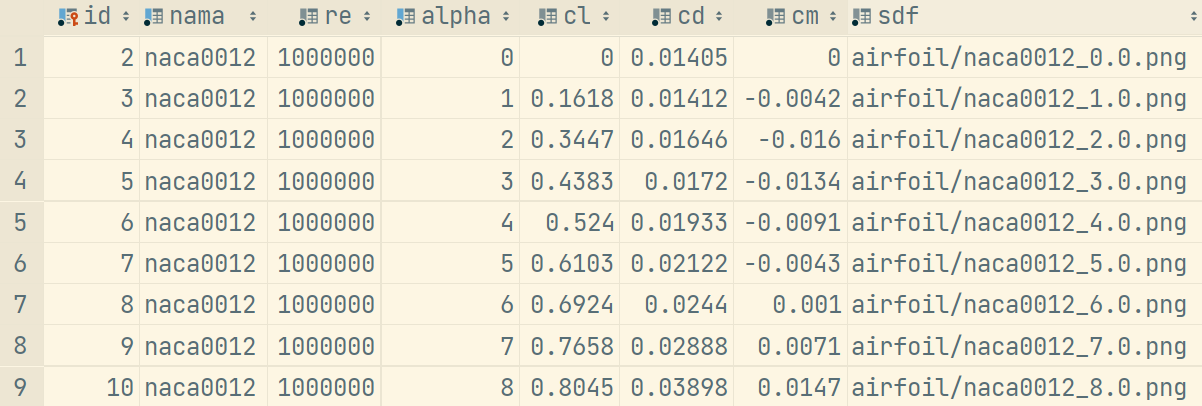
\includegraphics[width=0.7\linewidth]{statics/autoinsert}
  \end{figure}

\end{frame}
